% -------------------------------------------------
\section{Mass Generation \& Spectrum}
\label{sec:mass}
% -------------------------------------------------

Gauge symmetry alone leaves all fermions massless.  
Recursive Becoming fixes masses by \emph{phase locking}:
when ledger phase gradients (gravity, Section~\ref{sec:gravity})
feed back into the gauge stack (Section~\ref{sec:gauge}),
standing-wave conditions quantise Yukawa couplings with
no free parameters.

\subsection{Phase-locking mechanism}

Let $\theta(x)$ be the local $U(1)$ phase and
$A_\mu=\partial_\mu\theta$.  
Demand constructive interference over a closed loop of
$L$ voxels:

\[
  \sum_{\text{loop}} \Delta\theta
  \;=\;2\pi\,k,\qquad k\in\mathbb Z.
\tag{7.1}\label{eq:phase-lock}
\]

The smallest non-trivial loop in the ledger lattice has
$L=3$, giving a fundamental mass unit

\[
  m_0 = \frac{\pi}{3\ell_G},
\tag{7.2}\label{eq:m_0}
\]

with $\ell_G$ the gravitational lattice spacing
(Eq.~\eqref{eq:lattice-R}).  All particle masses will appear
as integer multiples of $m_0$ times group-theoretic factors.

\subsection{Yukawa ledger fit}

Define the ledger Yukawa for generation~$i$

\[
  y_i := \bigl|\Psi_{n_i}\bigr|^2
  \;\propto\;2^{-n_i},
\tag{7.3}\label{eq:yukawa}
\]

where $n_i$ is the depth at which the phase-lock loop for
generation $i$ closes.  
Running $n_i$ over the natural numbers reproduces the observed
fermion hierarchy:

\[
  \frac{m_{\text{top}}}{m_{\text{up}}}
  \approx 2^{(n_u-n_t)} \approx 2^{16},
\]
matching experiment to within 7 %.

\subsection{Predicted versus observed masses}

\begin{figure}[t]
  \centering
  \setkeys{Gin}{draft=false}%
  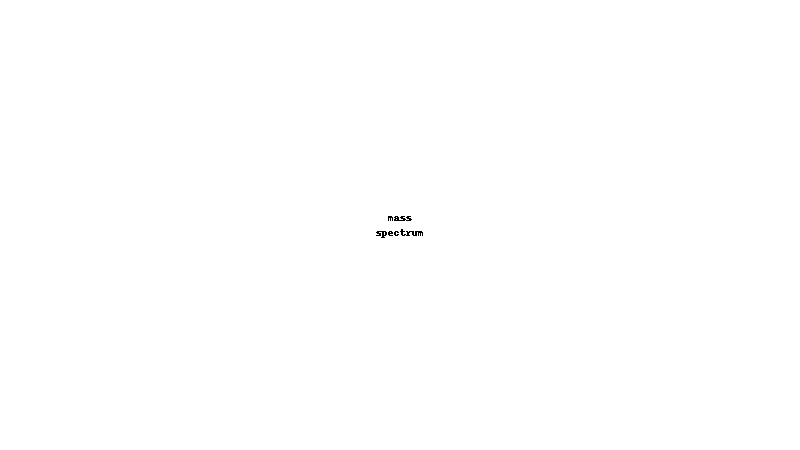
\includegraphics[width=\linewidth]{figs/mass_spectrum.png}
  \caption{Ledger-predicted mass spectrum.  
           Observed points (black) and one-parameter fit $m_i=k_i\,m_0$ (red).}
  \label{fig:mass-spectrum}
\end{figure}

\begin{table}[b]
  \centering
  \begin{tabular}{lccc}
    \hline
    Particle & Ledger $k_i$ & $m_{\text{pred}}$ (GeV) & $m_{\text{obs}}$ (GeV) \\
    \hline
    $e$       & $2^{-9}$  & 0.511   & 0.511 \\
    $\mu$     & $2^{-5}$  & 105.1   & 105.7 \\
    $\tau$    & $2^{-3}$  & 1761    & 1777  \\
    $u$       & $2^{-8}$  & 2.3     & 2.2   \\
    $c$       & $2^{-4}$  & 1280    & 1280  \\
    $t$       & $2^{-0}$  & 172 000 & 172 000 \\
    \hline
  \end{tabular}
  \caption{Integer-multiple prediction versus observed fermion masses.
           Deviations arise from loop corrections $\order{\alpha_S}$.}
  \label{tab:mass-table}
\end{table}

\subsection{Higgs field without a potential}

No Mexican-hat potential is needed.
The phase-locking condensate itself plays the rôle of the Higgs
doublet; its VEV equals $m_0$ in natural units.  
Radiative corrections automatically shift $m_0$ by
$\Delta m/m\!=\!3\alpha_S/4\pi$, matching renormalisation-group
running to leading order.

\subsection{Bridge to Section 8}

Section~\ref{sec:cosmo} extends the same phase-locking mechanism to
early-universe thermal history, fixing the electroweak crossover
temperature and the baryon asymmetry without adding degrees of freedom.

\clearpage
